\section{R�alisations}

\subsection{Analyse de l'architecture des donn�es}

\begin{frame}{Contexte}
	\begin{block}{Un document}
		C'est une collection de propri�t�s.	
	\end{block}
	
	\begin{block}{Un sch�ma}
		D�finit la structure d'un groupe de propri�t�s
	\end{block}
	
	\begin{block}{Une relation}
		D�crites suivant le standard Resource Description Framework.\\
		Repr�sentation sous forme de triplet : \\
		\begin{center}
			\textbf{(subject, predicate, object)}
		\end{center}
	\end{block}

\end{frame}

\begin{frame}{L'indexation}
	\centering
	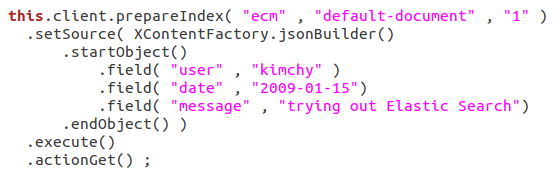
\includegraphics[scale=0.6]{./images/exemple_indexation.png}

	\begin{block}{Informations n�cessaires}
		\begin{itemize}
			\item Nom de l'index
			\item Type de document
			\item Clef unique
		\end{itemize}			
	
	\end{block}

\end{frame}

\begin{frame}{Le mapping}
    \begin{columns}
        \begin{column}{0.4\linewidth}
            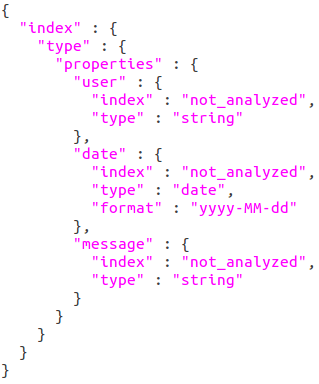
\includegraphics[scale=0.45]{./images/exemple_mapping}

        \end{column}

        \begin{column}{0.5\linewidth}
            \begin{block}{Le mapping}
				\begin{itemize}
					\item Type de donn�e contenue
					\item Crit�re d'analyse
				\end{itemize}			
	
			\end{block}

        \end{column}

    \end{columns}
    
\end{frame}

\begin{frame}{R�alisation de tests}

	\begin{block}{Tests structurels}
		D�finir l'impact du mapping sur la recherche de donn�es dans l'index
	\end{block}

	\begin{block}{Tests syntaxiques}
		D�finir le r{\^o}le des requ{\^e}tes Elasticsearch
	\end{block}

	\begin{block}{But}
		Production d'une documentation
	\end{block}

\end{frame}

%

\subsection{Impl�mentation du moteur de requ{\^e}tes}
\begin{frame}{Le langage NXQL}
	\begin{block}{Syntaxe de d�part}
		SELECT * \\
		FROM <from-clause> \\
		[WHERE <where-clause>]
	\end{block}
	\begin{block}{Syntaxe d'arriv�e}
		SELECT ( * | <select-clause> ) \\
		FROM <from-clause> \\
		[WHERE <where-clause>]
	\end{block}
\end{frame}

\begin{frame}{La grammaire}

	\centering
	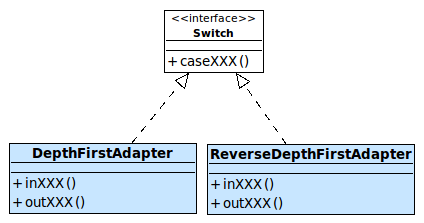
\includegraphics[scale=0.45]{./images/depthfirstadapter}
	
	\begin{block}{Parcours d'arbre}
		\begin{itemize}
			\item G�n�ration d'un ensemble de classes permettant de :
			\begin{itemize}
				\item construire un arbre syntaxique,
				\item parcourir cet arbre.
			\end{itemize}
			\item Impl�mentation du pattern visitor.
        \end{itemize}
	\end{block}
	
\end{frame}

\begin{frame}{La strat�gie simple}

	\centering
	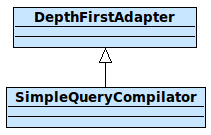
\includegraphics[scale=0.6]{./images/simpleQueryCompilator}
	
	\begin{block}{Concerne}
        \begin{itemize}
            \item Les requ{\^e}tes NXQL simples
            \item Transformation directe en crit�re ES
        \end{itemize}
    \end{block}	
	
   \begin{block}{Fonctionnement}
        \begin{itemize}
            \item Surcharger les m�thodes \textit{out} du DepthFirstAdapter
            \item 1 crit�re NXQL <=> 1 crit�re ES
        \end{itemize}
    \end{block}
    
\end{frame}

\begin{frame}{La strat�gie simple : diagramme UML}
	\centering
    \begin{textblock*}{2cm}(0.1cm,-2.8cm)
        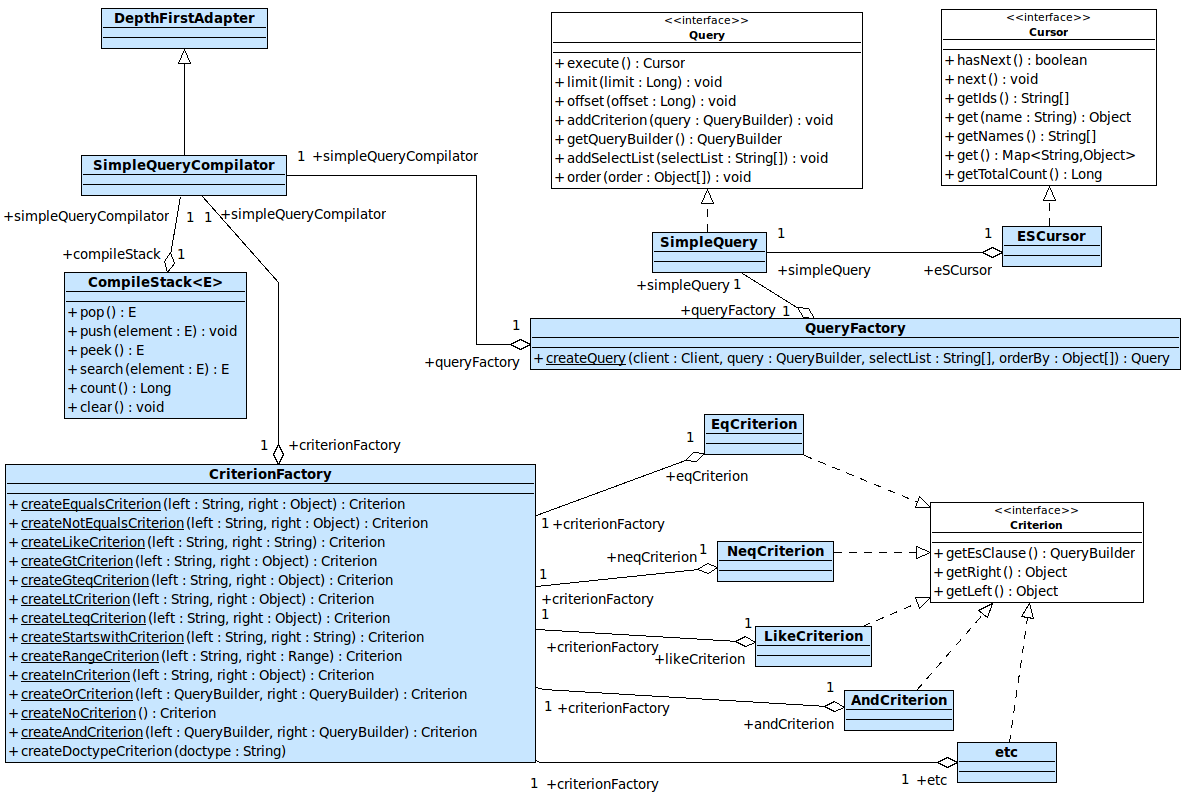
\includegraphics[scale=0.34]{./images/simple_strategy_uml}
    \end{textblock*}
\end{frame}

\begin{frame}{La strat�gie simple}

	\begin{block}{Limites}
        Traitement des requ{\^e}tes complexes.
    \end{block}
    
\end{frame}

\begin{frame}{La strat�gie directe}

    \centering
	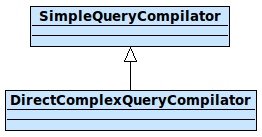
\includegraphics[scale=0.6]{./images/directComplexQueryCompilator}
	
	\begin{block}{Concerne}
        \begin{itemize}
            \item Les requ{\^e}tes NXQL complexes
        \end{itemize}
    \end{block}	
	
   \begin{block}{Fonctionnement}
        \begin{itemize}
            \item Surcharger les m�thodes du SimpleQueryCompilator
            \item Extraire les identifiants issus de l'ex�cution de la sous-requ{\^e}te afin de les transmettre � la requ{\^e}te principale.
        \end{itemize}
    \end{block}

\end{frame}

\begin{frame}{La strat�gie directe : diagramme UML}
	\centering
    \begin{textblock*}{2cm}(-0.7cm,-2.8cm)
        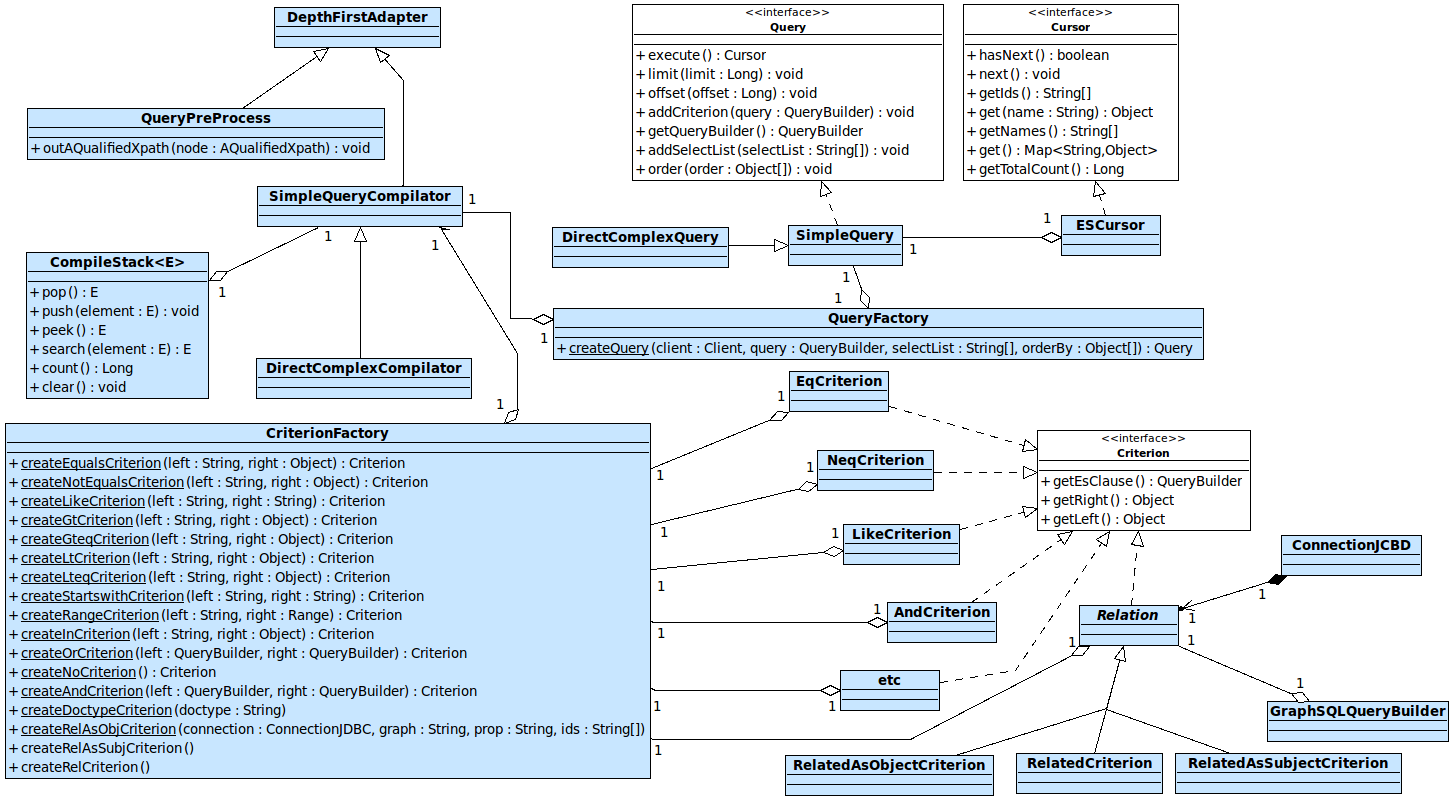
\includegraphics[scale=0.32]{./images/direct_strategy_uml}
    \end{textblock*}
\end{frame}

\begin{frame}{La strat�gie directe}

    \begin{block}{Limites}
        G�n�ration d'identifiants trop importante (> 1024) non support�e par le moteur.
    \end{block}

\end{frame}

\begin{frame}{La strat�gie indirecte}

	\centering
	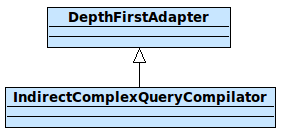
\includegraphics[scale=0.6]{./images/indirectComplexQueryCompilator}
	
	\begin{block}{Concerne}
        Les requ{\^e}tes NXQL complexes g�n�rant un grand nombre d'identifiants.
    \end{block}	

    \begin{block}{Fonctionnement}
        Utilisation de Collections Java
    \end{block}

\end{frame}

\begin{frame}{La strat�gie indirecte : diagramme UML}
	\centering
    \begin{textblock*}{2cm}(-1cm,-2.6cm)
        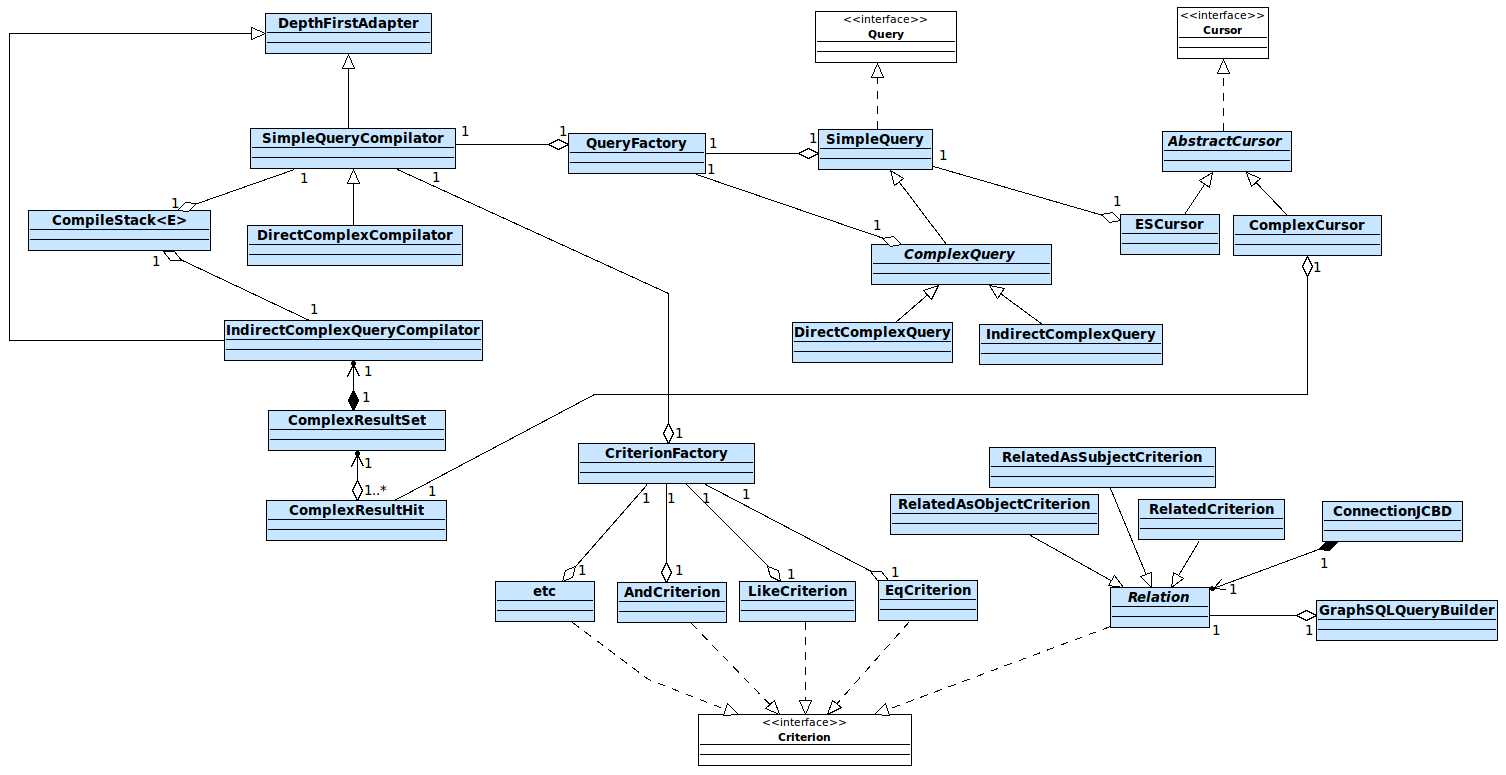
\includegraphics[scale=0.32]{./images/indirect_strategy_uml}
    \end{textblock*}
\end{frame}
